

%%%==================================================================================================
%%% PROBLEM STATEMENT
%%%==================================================================================================

A fundamental problem for torque-controlled humanoid robots is to accurately model their dynamics in presence of contacts, e.g., during manipulation in clutter~\cite{Jain2013}, whole-body movements~\cite{Kajita2008} or ground contacts in locomotion~\cite{Calandra2014}.
Analytic models suffer from inaccurate dynamic parameters, unmodeled dynamics (e.g., friction, couplings, elasticities) and noisy sensor measurements.
With contacts, the problem is even more challenging, because of discontinuities and additional non-linearities, which are difficult to model or estimate.
%One particular reason for this challenge is that
%contacts cause non-linearities in the system dynamics, which
%are difficult to model analytically or estimate. 
Moreover, if contact locations are not fixed a priori or known with sufficient precision, small errors in the localization of the external force can substantially deteriorate the quality of the inverse dynamics~\cite{DelPrete2012}.
%Additionally, analytic models suffer from inaccurate dynamic parameters, unmodeled dynamics (e.g., friction, couplings, elasticities) and noisy sensor measurements.
%play in the joints => can be solved kinematically

Nevertheless, many modern control strategies like inverse dynamics control~\cite{Erez2012}, computed torque control~\cite{Siciliano2009} or model predictive control approaches~\cite{Naveau2014} rely on accurate dynamic models.
% too risky: there are techniques in NMPC that do not need this 
%(or even differentiable) dynamics models.
With inaccurate dynamics models these control strategies can produce suboptimal policies, by not taking the external forces (caused by contacts) into account, and even damages to the hardware.

%%%==================================================================================================
%%% OUR CONTRIBUTION
%%%==================================================================================================
%
\begin{wrapfigure}{r}{0.30\columnwidth}
%\begin{figure}[t]
	\vspace{-10pt}
	\centering
	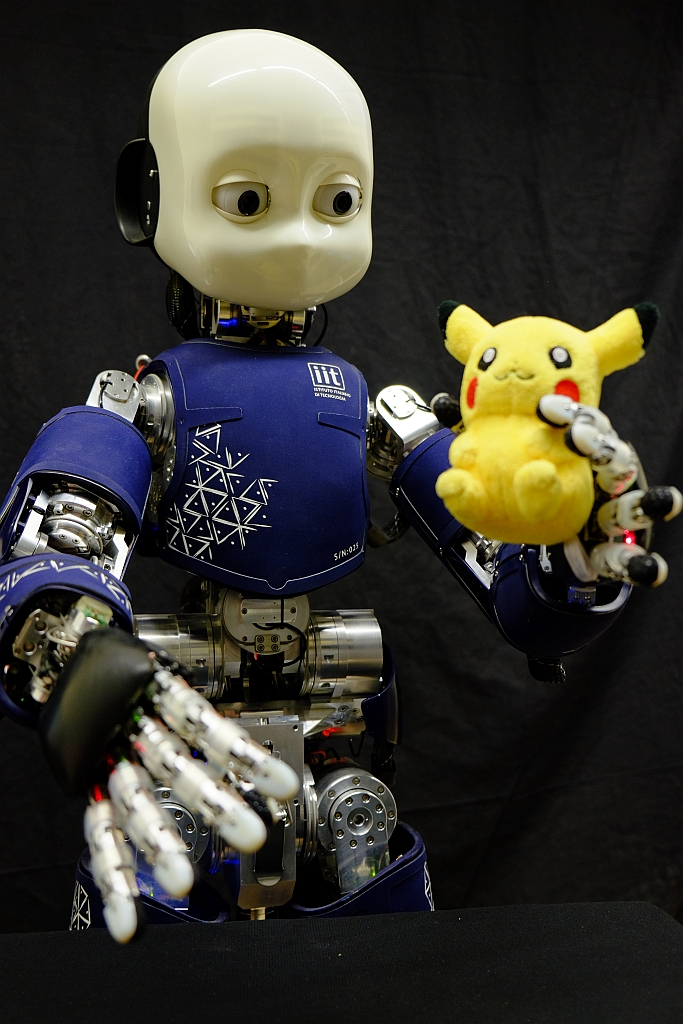
\includegraphics[width=.999\linewidth]{robertoIROS/fig/iCubDarmstadt01_new}
	\caption{The humanoid robot \robot{} used in the experiments.}
    \vspace{-10pt}
	\label{fig:icub}
%\end{figure}
\end{wrapfigure}
%
%%-------------------------------------
%% Our approach
%%-------------------------------------
%
%As a first step toward a more informed controller that explicitly considers the effect of contacts, we propose to learn the dynamics model from tactile sensor readings and force-torque sensors. 
In contrast to classical techniques based on the identification of dynamics parameters~\cite{Yamane2011calibration,Ogawa2014,Traversaro2013}, we propose a fully data-driven machine learning approach based on non-parametric models, where both the rigid body dynamics as well as the effect of external forces on the robot structure are learned directly from data collected on the real robot.
The proposed model makes use of the raw sensory data and does not require a kinematic/dynamics calibration~\cite{Yamane2011calibration,Ogawa2014,Traversaro2013}: in particular, it does not need a spatially calibrated model of the skin~\cite{DelPrete2011}.
As a non-linear model for the inverse dynamics we propose to learn a ``mixtures of contacts'' based on Gaussian Processes (GP).
%Each of these GP experts models a single ``type'' of contact and can be easily learned.
%However, by using a gating network that activates and deactivates the individual GP experts, it is %possible to switch between contacts and generalize to more complex environments.
% \todo[inline, color=yellow]{I don't think this bit is necessary here...\\
% As ground-truth we use joint-torque sensor measurements,
% and  we compare to a state-of-the-art analytic modeling approach
% that assumes perfect knowledge of the contact location to model external forces.
% Our approach in contrast, uses simply the tactile information to activate the experts.}
% The Gaussian processes are trained with the robot configurations (in joint angles)
% and the force measurements of the joint-torque sensors.
%
%
%============================================================
% CHANGE ME
%

%%-------------------------------------
%% Experimental results
%%-------------------------------------
%

We evaluate our model learning approach on two different tasks using the arm of the \robot{} humanoid robot~\cite{Natale2013} (see \fig\ref{fig:icub}) and compare against a state-of-the-art analytic modeling approach.
%The learned inverse dynamics model outperforms the analytic approach and we demonstrate that the model can generalize to new environmental conditions, such as changing contact locations.
%To the best of our knowledge, this is the first demonstration of how joint torques can be learned on a humanoid robot equipped with tactile and force/torque sensors in presence of contacts.
%
% 
In the first task, the learned inverse dynamics is used to compensate for an unexpected obstruction and minimize the tracking error.
In the second task, we use the learned model on a controller designed to slide along an obstruction. 
The purpose of the sliding controller is to minimize the contact forces and therefore avoid to break the motors or the artificial tendons that actuate the joints in the case of unexpected contacts.


